\section{Freiman's constant. Initial set of rectangles}

All these rectangles satisfy \textit{\_here will be a complete list of conditions.\_}

At least all of them are good, in terms of section \oldref{section_good}.

%Their projections, in terms of section \oldref{section_boundaries}, cover the beginning of Hall's Ray.

\begin{figure}[H]
	\centering
	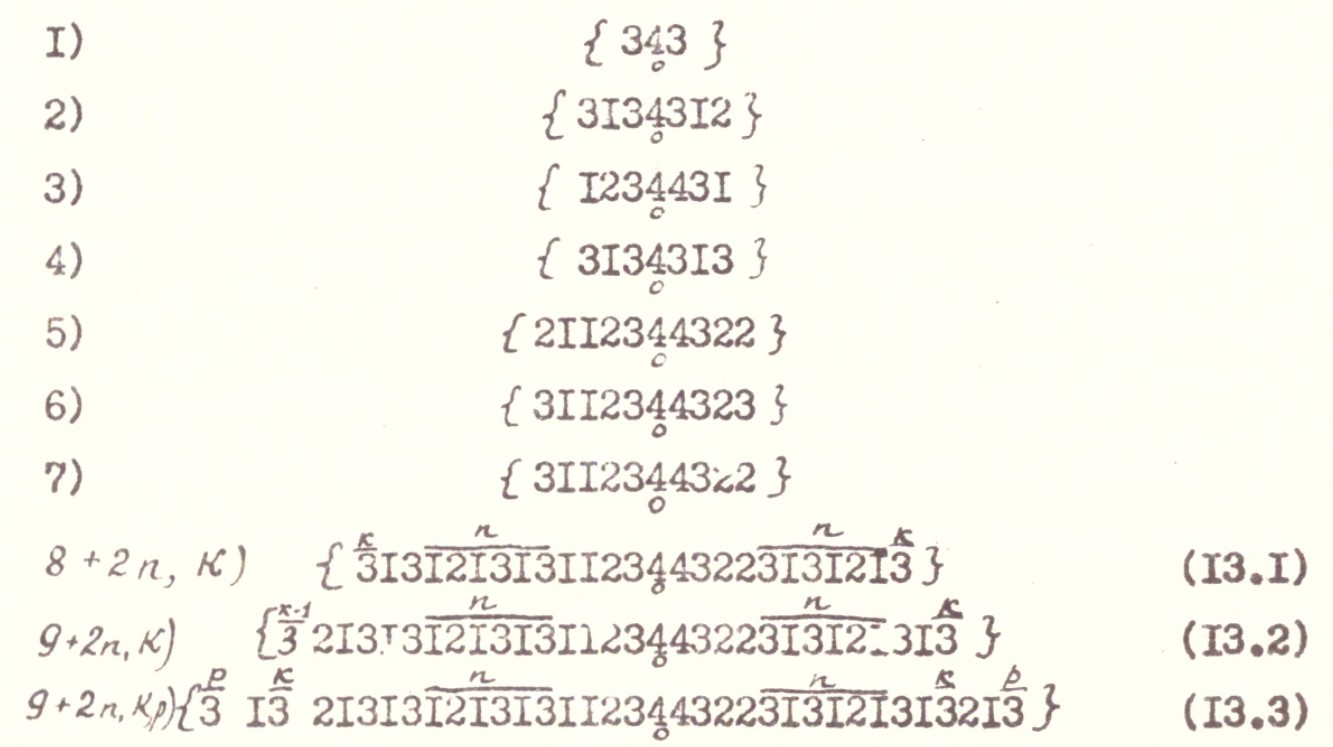
\includegraphics[width=0.8\textwidth]{initial_set}
	\caption{Freiman's constant. Initial set of rectangles.}
	\label{fc_init}
\end{figure}
